\chapter{METODE PENELITIAN}

\vspace{1cm}
\section{Tahapan Penelitian}
\hspace{1,2cm}Berdasarkan rumusan masalah, pada dasarnya kegiatan penelitian ilmiah ini terdapat beberapa tahap yang dijelaskan pada Gambar \ref{img:Tahapan-Penelitian}, warna hijau pada diagram adalah kebaruan (\textit{novelty}).

%%%%%%%%%%%%%%%%%%%%%%%%%% GAMBAR %%%%%%%%%%%%%%%%%%%%%%%%%%%%%%
\begin{figure}[H]
	\vspace{-0.1cm}
	%\rule{\columnwidth}{0.1pt}
	\begin{center}
		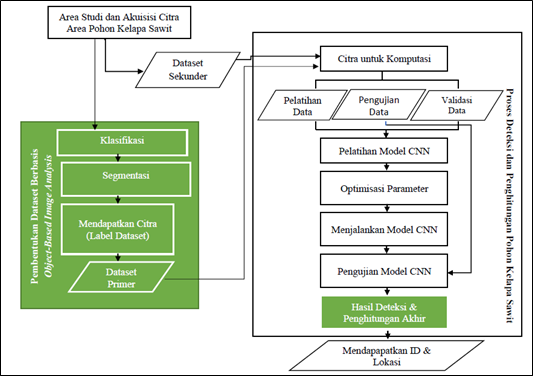
\includegraphics[width=1\columnwidth]{bab3/Gambar/Picture1.png}
	\end{center}
	\vspace{-0.2cm}
	%\rule{\columnwidth}{0.1pt}
	\captionsetup{justification=centering}
	\caption{Tahapan Penelitian yang Dilakukan}\label{img:Tahapan-Penelitian}
\end{figure}
%%%%%%%%%%%%%%%%%%%%%%%%%% GAMBAR %%%%%%%%%%%%%%%%%%%%%%%%%%%%%%

Penelitian ini secara umum digambarkan pada Gambar \ref{img:Tahapan-Penelitian}. Dimulai dari studi area dan akusisi citra area kelapa sawit yang merupakan gambaran dimana citra data terbentuk untuk mendapatkan dataset primer dan dataset sekunder untuk dapat digunakan sebagai citra untuk komputasi. Penelitian ini mengusulkan data citra primer yang didapat dari citra drone dengan pendekatan \textit{object-based image analysis} (OBIA). Pendekatan OBIA untuk dihasilkan citra dengan otomasi dataset atau data citra yang belum diberikan label atau anotasi sebuah kelas, dapat dilakukan anotasi atau pemberikan label kelas pohon kelapa sawit secara otomatis, tidak dilakukan anotasi data citra satu per satu. Pendeketan ini dengan menggunakan proses klasifikasi dan segmentasi yang merupakan kunci dari proses pendekatan OBIA. Dataset yang terbentuk digabungkan dengan dataset sekunder yang digunakan untuk menambahdata. Data tersebut merupakan gambar atau citra yang sudah memiliki label atau anotasi untuk menjadi citra yang digunakan untuk komputasi. Citra tersebut terbagi menjadi tiga, yaitu citra data untuk pelatihan, validasi, dan pengujian dengan model CNN untuk mendeteksi dan menghitung citra pohon kelapa sawit, kemudian model digunakan dalam sistem yang terintergrasi secara real-time, sehingga dapat mendeteksi dna menghitung kepala sawit, serta mengetahui dan mendapatkan identitas dan letak posisi koordinat (latitude dan longitude) setiap pohon kelapa sawit yang berhaisl terdeteksi.

\section{Area Studi Penelitian Kelapa Sawit}
\hspace{1,2cm}Penelitian ini dilakukan di Indonesia yang berada pada lokasi Kebun Pendidikan dan Penelitian Kelapa Sawit milik Institut Pertanian Bogor-Cargil yang berlokasi di Jonggol, Jawa Barat dan Universitas Gunadarma di Kalimantan yang memiliki lahan yang ditumbuhi pohon kelapa sawit. Hasil lahan perbekunan pohon kelapa sawit ini berupa citra yang diambil dari drone dengan jenis DJI Mavic 2 Pro dari ketinggian 100 m di atas permukaan tanah. Kebun Pendidikan dan Penelitian Kelapa Sawit IPB-Cargil juga dijadikan untuk pengujian penerapan sistem yang diusulkan dalam penelitian ini. Lokasi Kebun Pendidikan dan Penelitian kelapa Sawit tersebut berada pada latitude -6.4277942 dan longitude 106.8418378, sedangkan lokasi di Universitas Gunadarma PPU Campus berada pada latitude -1.318495 dan longitude 116.6678405. Luas dari kebun pohon kelapa sawit yang berada pada IPB-Cargil berdasarkan studi lapang dan perhitungan dengan DroneDeploy ini seluas 63,48 hektar, dan untuk luas wilayah yang ditanami pohon kelapa sawit pada lahan yang dimiliki Universitas Gunadarma berdasarkan hasil wawancara seluas $\approx$ 18 hektar. Gambar 3.2. dan 3.3. menampilkan posisi studi area dari penelitian ini.

%%%%%%%%%%%%%%%%%%%%%%%%%% GAMBAR %%%%%%%%%%%%%%%%%%%%%%%%%%%%%%
\begin{figure}[H]
	\vspace{-0.1cm}
	%\rule{\columnwidth}{0.1pt}
	\begin{center}
		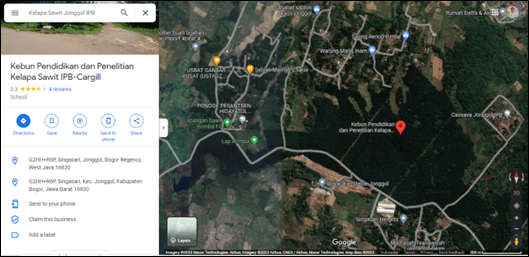
\includegraphics[width=1\columnwidth]{bab3/Gambar/Picture2.png}
	\end{center}
	\vspace{-0.2cm}
	%\rule{\columnwidth}{0.1pt}
	\captionsetup{justification=centering}
	\caption{Lokasi Kebun Pendidikan dan Penelitian Kelapa Sawit IPB-Cargil}\label{img:Lokasi-Kebun-IPB}
\end{figure}
%%%%%%%%%%%%%%%%%%%%%%%%%% GAMBAR %%%%%%%%%%%%%%%%%%%%%%%%%%%%%%

%%%%%%%%%%%%%%%%%%%%%%%%%% GAMBAR %%%%%%%%%%%%%%%%%%%%%%%%%%%%%%
\begin{figure}[H]
	\vspace{-0.1cm}
	%\rule{\columnwidth}{0.1pt}
	\begin{center}
		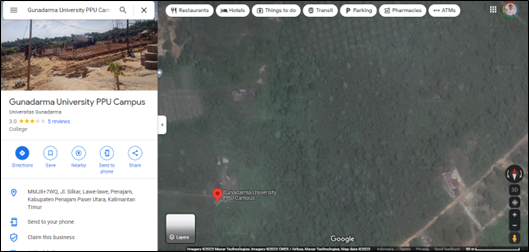
\includegraphics[width=1\columnwidth]{bab3/Gambar/Picture3.png}
	\end{center}
	\vspace{-0.2cm}
	%\rule{\columnwidth}{0.1pt}
	\captionsetup{justification=centering}
	\caption{Lokasi Universitas Gunadarma PPU Campus yang ditanami Pohon Kelapa Sawit}\label{img:Lokasi-Gunadarma}
\end{figure}
%%%%%%%%%%%%%%%%%%%%%%%%%% GAMBAR %%%%%%%%%%%%%%%%%%%%%%%%%%%%%%

\section{Persiapan Data}
\hspace{1,2cm}Persiapan data atau yang dikenal dengan \textit{data preprocessing} merupakan tahap untuk menyiapkan atau mengubah data awal dan siap untuk dapat digunakan dalam menjalankan proses modeling pada \textit{deep learning}. Tahap ini digunakan berdasarkan \textit{data mining life cycle} atau siklus hidup data mining yang dikemukakan oleh Cross-Industry Standard Process for Data Mining (CRISP-DM) Nvidia. Salah satu proses tersebut untuk membangun data dengan pembangunan dataset berbasis OBIA, sehingga proses anotasi atau pelabelan secara otomatis menjadi lebih cepat yang menjadi salah satu kebaruan dari penelitian ini. Adapun diagram persiapan data pada penelitian ini pada Gambar 3.4.

%%%%%%%%%%%%%%%%%%%%%%%%%% GAMBAR %%%%%%%%%%%%%%%%%%%%%%%%%%%%%%
\begin{figure}[H]
	\vspace{-0.1cm}
	%\rule{\columnwidth}{0.1pt}
	\begin{center}
		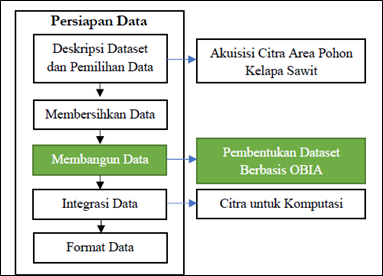
\includegraphics[width=0.6\columnwidth]{bab3/Gambar/Picture4.png}
	\end{center}
	\vspace{-0.2cm}
	%\rule{\columnwidth}{0.1pt}
	\captionsetup{justification=centering}
	\caption{Diagram Proses Persiapan Data}\label{img:Diagram-Proses-Persiapan-Data}
\end{figure}
%%%%%%%%%%%%%%%%%%%%%%%%%% GAMBAR %%%%%%%%%%%%%%%%%%%%%%%%%%%%%%

\subsection{Deskripsi Dataset dan Pemilihan Data}
\hspace{1,2cm}Pada bagian ini merupakan deskripsi dataset dan pemilihan data yang berisi akuisisi citra area pohon kelapa sawit yang digunakan sebagai dataset untuk citra komputasi. Akuisisi citra ini merupakan proses menangkap atau memindai dari alat yang digunakan untuk menjadi suatu citra atau gambar. Citra area pohon kelapa sawit dibagi menjadi dua, yaitu citra dataset primer dan sekunder. Setiap gambar di dataset memiliki format *.jpg.

\begin{enumerate}
	\item Dataset Primer
	
	Dataset primer yang digunakan data yang dikumpulkan langsung dari sumber data langsung tanpa melalui sumber yang sudah ada atau disediakan. Dataset primer ditangkap dengan menggunakan sarana penelitian drone DJI Mavic 2 Pro dari 100 m di atas permukaan tanah. Dataset ini dijadikan sebagia dataset yang diambil secara langsung untuk digunakan sebagai dataset primer yang belum memiliki label atau anotasi objek kelapa sawit di dalam suatu citra yang ditangkap oleh drone. Citra yang dihasilkan dari area kampus Universitas Gunadarma - PPU dihasilkan 205 gambar dengan dimensi masing-masing sebesar 5472 x 3078 dengan format *.jpg, dan gambar citra pohon kelapa sawit di area tersebut seperti pada Gambar \ref{img:Hasil-Citra-Area-Pohon}.
	
	%%%%%%%%%%%%%%%%%%%%%%%%%% GAMBAR %%%%%%%%%%%%%%%%%%%%%%%%%%%%%%
	\begin{figure}[H]
		\vspace{-0.1cm}
		%\rule{\columnwidth}{0.1pt}
		\begin{center}
			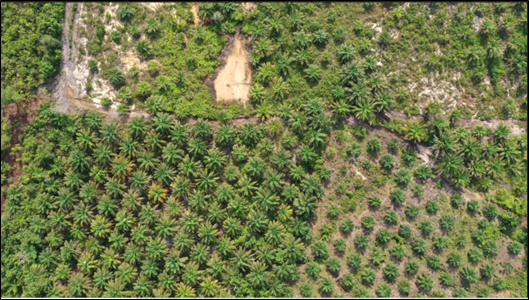
\includegraphics[width=1\columnwidth]{bab3/Gambar/Picture5.png}
		\end{center}
		\vspace{-0.2cm}
		%\rule{\columnwidth}{0.1pt}
		\captionsetup{justification=centering}
		\caption{Hasil Citra Area Pohon Kelapa Sawit PPU untuk Dataset Primer}\label{img:Hasil-Citra-Area-Pohon}
	\end{figure}
	%%%%%%%%%%%%%%%%%%%%%%%%%% GAMBAR %%%%%%%%%%%%%%%%%%%%%%%%%%%%%%
	
	Citra yang dihasilkan dari area Kebun Pendidikan dan Penelitian Kelapa Sawit IPB-Cargil diambil dari area blok 3 dan blok 4 dengan drone DJI Mavic 2 Pro dari ketinggian 100 m di atas permukaan tanah. Luas area dari blok 3 dan blok 4 berdasarkan perhitungan dengan bantuan layanan DroneDeploy, seperti pada Tabel \ref{tbl:Luas-Area-Dari-Gambar-Citra}.
	
	%%%%%%%%%%%%%%%%%%%%%%%TABEL SEDERHANA%%%%%%%%%%%%%%%%%%%%%%%%%
	\begin{singlespace}
		\begin{table}[H]
			\centering
			\caption{Luas Area Dari Gambar Citra yang Ditangkap oleh drone di Kebun Pendidikan dan Penelitian Kelapa Sawit IPB-Cargil}
			\label{tbl:Luas-Area-Dari-Gambar-Citra}
			\begin{tabular}{|cc|c|}
				\hline
				\multicolumn{1}{|c|}{No.} & Area   & Luas Area (ha) \\ \hline
				\multicolumn{1}{|c|}{1}   & Blok 3 & 18,20          \\ \hline
				\multicolumn{1}{|c|}{2}   & Blok 4 & 19,31          \\ \hline
				\multicolumn{2}{|c|}{Total}        & 37,51          \\ \hline
			\end{tabular}
		\end{table}
	\end{singlespace}
	%%%%%%%%%%%%%%%%%%%%%%%TABEL SEDERHANA%%%%%%%%%%%%%%%%%%%%%%%%%
	
	Studi lapang dengan mengambil gambar bisa mencakup area 37,51 hektar dari blok 3 dan 4 blok dari total 4 blok yang tersedia. Berikut ini hasil tangkapan citra dari Kebun Pendidikan dan Penelitian Kelapa Sawit IPB-Cargil pada Gambar \ref{img:Hasil-Citra-Blok-3} untuk blok 3 dengan dimensi gambar 32356 x 31214 dan Gambar \ref{img:Hasil-Citra-Blok-4}. untuk blok 4, dengan dimensi gambar 43684 x 23452 dengan format *.jpg.
	
	%%%%%%%%%%%%%%%%%%%%%%%%%% GAMBAR %%%%%%%%%%%%%%%%%%%%%%%%%%%%%%
	\begin{figure}[H]
		\vspace{-0.1cm}
		%\rule{\columnwidth}{0.1pt}
		\begin{center}
			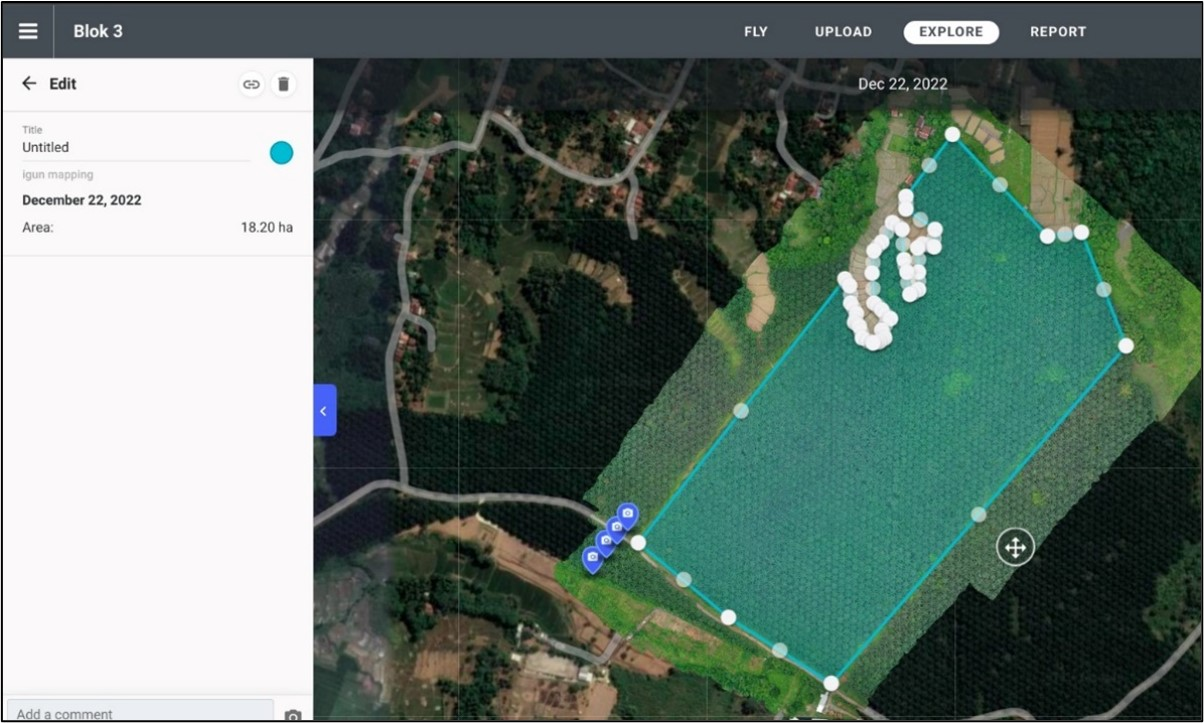
\includegraphics[width=1\columnwidth]{bab3/Gambar/Picture6.jpg}
		\end{center}
		\vspace{-0.2cm}
		%\rule{\columnwidth}{0.1pt}
		\captionsetup{justification=centering}
		\caption{Hasil Citra Blok 3 untuk Dataset Primer (luas area dalam ha)}\label{img:Hasil-Citra-Blok-3}
	\end{figure}
	%%%%%%%%%%%%%%%%%%%%%%%%%% GAMBAR %%%%%%%%%%%%%%%%%%%%%%%%%%%%%%
	
	%%%%%%%%%%%%%%%%%%%%%%%%%% GAMBAR %%%%%%%%%%%%%%%%%%%%%%%%%%%%%%
	\begin{figure}[H]
		\vspace{-0.1cm}
		%\rule{\columnwidth}{0.1pt}
		\begin{center}
			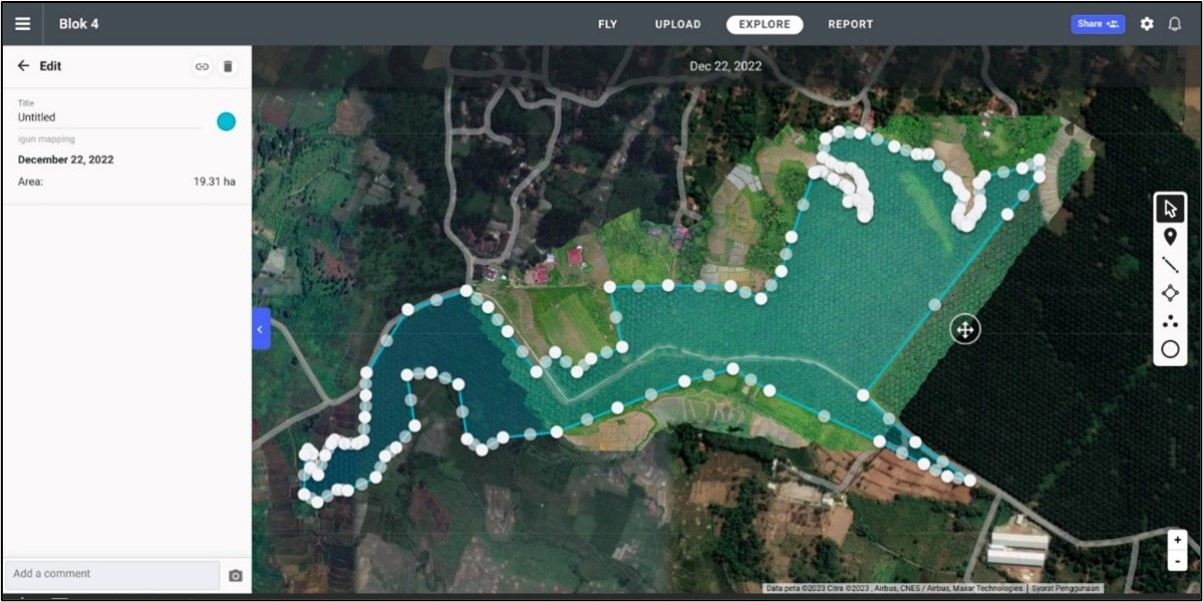
\includegraphics[width=1\columnwidth]{bab3/Gambar/Picture7.jpg}
		\end{center}
		\vspace{-0.2cm}
		%\rule{\columnwidth}{0.1pt}
		\captionsetup{justification=centering}
		\caption{Hasil Citra Blok 4 untuk Dataset Primer (luas area dalam ha)}\label{img:Hasil-Citra-Blok-4}
	\end{figure}
	%%%%%%%%%%%%%%%%%%%%%%%%%% GAMBAR %%%%%%%%%%%%%%%%%%%%%%%%%%%%%%
	Dataset primer ini digunakan untuk pembentukan dataset yang dibentuk secara ototamatis dalam proses anotasi atau memberikan label kepada objek kelapa sawit pada citra file yang terdeteksi tanpa harus melakukan proses anotasi atau pemberian label kelapa sawit satu persatu. Proses ini dilakukan pada bagian sub bab 3.3.3. sebagai salah satu kebaruan atau \textit{novelty} yang diusulkan.
	
	\item Dataset Sekunder
	
	Data sekunder yang digunakan merupakan data citra yang sudah memiliki label atau anotasi sebagai pohon kelapa sawit (oil palm), dan dikatakan sebagai dataset. Data yang digunakan dalam penelitian ini diambil dari 1795 citra satelit sentinel 2 dari roboflow (JS, 2022). Dataset yang sudah diberikan label dengan memiliki kotak atau bounding box. Dataset ini masing-masing memiliki dimensi citra gambar 1024 x 1024 dengan format file *.jpg. Dataset sekunder yang sudah diberikan anotasi atau label oil palm diakses melalui roboflow, seperti pada Gambar \ref{img:Data-Sekunder-yang-Sudah-Diberikan-Label}. 
	
	%%%%%%%%%%%%%%%%%%%%%%%%%% GAMBAR %%%%%%%%%%%%%%%%%%%%%%%%%%%%%%
	\begin{figure}[H]
		\vspace{-0.1cm}
		%\rule{\columnwidth}{0.1pt}
		\begin{center}
			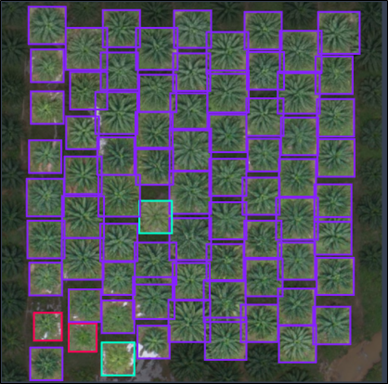
\includegraphics[width=1\columnwidth]{bab3/Gambar/Picture8.png}
		\end{center}
		\vspace{-0.2cm}
		%\rule{\columnwidth}{0.1pt}
		\captionsetup{justification=centering}
		\caption{Data sekunder yang sudah Diberikan Label atau Anotasi Oil Palm\\(Sumber: JS, 2022)}\label{img:Data-Sekunder-yang-Sudah-Diberikan-Label}
	\end{figure}
	%%%%%%%%%%%%%%%%%%%%%%%%%% GAMBAR %%%%%%%%%%%%%%%%%%%%%%%%%%%%%%
	
	Pada data sekunder ditambah untuk mendapatkan lebih banyak citra dan representasi dengan menambahkan citra menjadi 3987 citra dengan melakukan augmentasi seperti pada Tabel \ref{tbl:Augmentasi-Dataset-Sekunder}.
	
	%%%%%%%%%%%%%%%%%%%%%%%TABEL SEDERHANA%%%%%%%%%%%%%%%%%%%%%%%%%
	\begin{singlespace}
		\begin{table}[H]
			\centering
			\caption{Augmentasi Dataset Sekunder untuk Menambahkan Data}
			\label{tbl:Augmentasi-Dataset-Sekunder}
			\begin{tabular}{|p{4cm}|p{8cm}|}
				\hline
				Augmentasi & Deskripsi                           \\ \hline
				
				Crop       & 0\% Minimum Zoom, 40\% Maximum Zoom \\ \hline
				
				Rotation   & Between -39$^{\circ}$ and +39$^{\circ}$               \\ \hline
				Hue & Between -30$^{\circ}$ and +3$^{\circ}$\\ \hline
				
				Exposure & Between -17$^{\circ}$ and +17$^{\circ}$ \\ \hline
				
				Blur & Up to 2.5px \\ \hline
				
				Noise & Up to 2\% of pixels \\ \hline
				
				Mosaic & Applied \\ \hline
			\end{tabular}
		\end{table}
	\end{singlespace}
	%%%%%%%%%%%%%%%%%%%%%%%TABEL SEDERHANA%%%%%%%%%%%%%%%%%%%%%%%%%
	
	Proses Tabel \ref{tbl:Augmentasi-Dataset-Sekunder}. dilakukan pada roboflow. Roboflow merupakan sebuah platform yang memfasilitasi proses anotasi dataset dan juga menyimpan data citra. Untuk data citra primer yang digunakan menggunakan drone DJI Mavic 2 Pro yang diambil dari Perkebunan Kelapa Sawit Institut Pertanian Bogor yang terletak di Jonggol dan di Universitas Gunadarma Kalimantan. Dataset primer yang diambil di Universitas Gunadarma di Kalimantan menghasilkan 205 citra, sedangkan data citra primer yang diambil dari Jonggol, Jawa Barat pada blok 3 dan 4 dipecah, sehingga menghasilkan 69 citra seperti yang ditunjukkan pada Gambar \ref{img:Gambar-Dataset-Sekunder}.
	
	%%%%%%%%%%%%%%%%%%%%%%%%%% GAMBAR %%%%%%%%%%%%%%%%%%%%%%%%%%%%%%
	\begin{figure}[H]
		\vspace{-0.1cm}
		%\rule{\columnwidth}{0.1pt}
		\begin{center}
			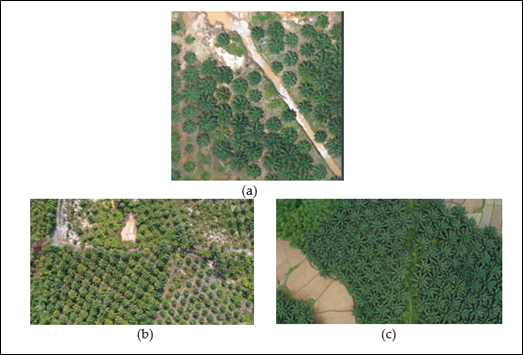
\includegraphics[width=1\columnwidth]{bab3/Gambar/Picture9.png}
		\end{center}
		\vspace{-0.2cm}
		%\rule{\columnwidth}{0.1pt}
		\captionsetup{justification=centering}
		\caption{(a) Gambar Dataset Sekunder; (b) Gambar Dataset Primer di Kalimantan; (c) Gambar Dataset Primer di Jonggol;.}\label{img:Gambar-Dataset-Sekunder}
	\end{figure}
	%%%%%%%%%%%%%%%%%%%%%%%%%% GAMBAR %%%%%%%%%%%%%%%%%%%%%%%%%%%%%%
\end{enumerate}

\subsection{Membersihkan Data}
Bagian ini dikenal dengan \textit{clean data} atau membersihkan data. Pada penelitian ini yang dilakukan pada tahap membersihkan data adalah memvalidasi citra yang ditangkap oleh drone berada pada tangkapan citra yang tegak, tidak diambil dari sisi samping dari kamera drone untuk menjaga keseragaman data yang dimiliki pada dataset, serta dilihat juga apakah gambar tersebut memiliki tangkapan citra pohon kelapa sawit atau tidak, seperti pada Gambar 3.10.

%%%%%%%%%%%%%%%%%%%%%%%%%% GAMBAR %%%%%%%%%%%%%%%%%%%%%%%%%%%%%%
\begin{figure}[H]
	\vspace{-0.1cm}
	%\rule{\columnwidth}{0.1pt}
	\begin{center}
		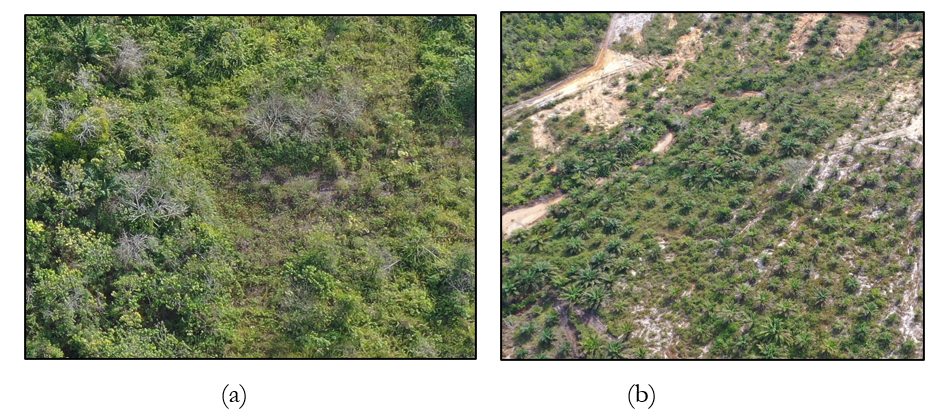
\includegraphics[width=1\columnwidth]{bab3/Gambar/Picture10.png}
	\end{center}
	\vspace{-0.2cm}
	%\rule{\columnwidth}{0.1pt}
	\captionsetup{justification=centering}
	\caption{Citra yang tidak digunakan sebagai dataset (a) tidak ada pohon citra kelapa sawit; (b) tangkapan citra dari drone tidak dari sisi atas yang tegak}\label{img:Citra-Yang-Tidak-Digunakan}
\end{figure}
%%%%%%%%%%%%%%%%%%%%%%%%%% GAMBAR %%%%%%%%%%%%%%%%%%%%%%%%%%%%%%

\subsection{Membangun Data}
\hspace{1,2cm}Persiapan dan pemahaman data dari data primer dan sekunder merupakan tugas paling penting. Tugas ini membutuhkan dan menghabiskan waktu hampir 70\% waktunya untuk menganalisis kumpulan data. Tugas yang dilakukan dalam dataset diantaranya persiapan dan pemahaman data, seperti memberi anotasi atau label pada data atau dengan istilah lain membangun data (\textit{construct data}). Selama ini, dalam melakukan anotasi atau pemberian label dilakukan masih manual atau memberikan tanda kotak (\textit{bounding box}) untuk setiap data atau objek pada gambar yang ditandai sebagai dataset. Maka, dibutuhkan suatu pendekatan untuk melakukan anotasi atau labelisasi secara otomatis, yaitu pembentukan dataset berbasis \textit{object-based image analysis} (OBIA). Pendekatan dalam penelitian ini menggunakan OBIA. Secara umum OBIA menawarkan sebuah alternatif untuk pemrosesan citra berbasis objek. Mengekstrak informasi tutupan lahan/penggunaan lahan yang merupakan tantangan baru, tetapi dengan prinsip dasar klasifikasi dan segmentasi dapat digunakan untuk membuat dataset secara otomatis. Dataset yang digunakan berupa gambar primer yang sudah dimiliki berasal data tangkap citra drone. Algoritma \textit{template matching} dan \textit{balanced iterative reducing and clustering using hierarchies} (BIRCH) dapat digunakan untuk pengenalan gambar, yaitu membandingkan dua atau lebih gambar yang identik pada waktu dan kondisi yang berbeda, sehingga dapat menyaring objek dengan nilai ambang batas atau (thereshold) dan membentuk \textit{fine tuning} atau nilai yang lebih baik untuk dapat dideteksi secara otomatis. Pembentukan atau pemberian label dengen pendekatan OBIA inilah menjadi kebaruan atau \textit{novelty} untuk mendukung proses tersebut menjadi lebih cepat dan signifikan dalam pemberian label atau anotasi pada dataset citra.

Pengembangan sistem untuk membangun dataset dengan anotasi atau label otomatis dengan sarana penelitian seperti pada Tabel \ref{tbl:Sarana-Penelitian-Pengembangan-Sistem-Untuk-Membangun-Dataset}.

%%%%%%%%%%%%%%%%%%%%%%%TABEL SEDERHANA%%%%%%%%%%%%%%%%%%%%%%%%%
\begin{singlespace}
	\begin{table}[H]
		\centering
		\caption{Sarana Penelitian Pengembangan Sistem untuk Membangun Dataset dengan Anotasi atau Label Otomatis}
		\label{tbl:Sarana-Penelitian-Pengembangan-Sistem-Untuk-Membangun-Dataset}
		\begin{tabular}{|c|c|}
			\hline
			Alat                  & Keterangan                        \\ \hline
			Drone                 & DJI Mavic 2 Pro                   \\ \hline
			Jupyter Notebook      & V 6.4.11                          \\ \hline
			Python                & Python 3                          \\ \hline
			OS Name               & Microsoft Windows 10 Pro          \\ \hline
			Processor             & Intel Core i5-6300U CPU @2.40 GHz \\ \hline
			Phsyical Memory (RAM) & 8,00 GB                           \\ \hline
		\end{tabular}
	\end{table}
\end{singlespace}
%%%%%%%%%%%%%%%%%%%%%%%TABEL SEDERHANA%%%%%%%%%%%%%%%%%%%%%%%%%

Diagram alur untuk membuat dataset otomatis seperti pada Gambar \ref{img:Diagram-Alir-Pembangunan-Dataset}

%%%%%%%%%%%%%%%%%%%%%%%%%% GAMBAR %%%%%%%%%%%%%%%%%%%%%%%%%%%%%%
\begin{figure}[H]
	\vspace{-0.1cm}
	%\rule{\columnwidth}{0.1pt}
	\begin{center}
		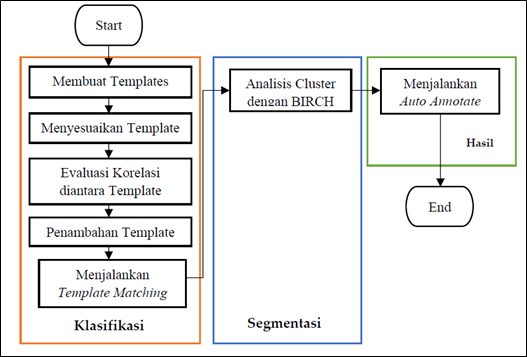
\includegraphics[width=1\columnwidth]{bab3/Gambar/Picture11.png}
	\end{center}
	\vspace{-0.2cm}
	%\rule{\columnwidth}{0.1pt}
	\captionsetup{justification=centering}
	\caption{Diagram Alir Pembangunan Dataset Berdasarkan Pendekatan OBIA}\label{img:Diagram-Alir-Pembangunan-Dataset}
\end{figure}
%%%%%%%%%%%%%%%%%%%%%%%%%% GAMBAR %%%%%%%%%%%%%%%%%%%%%%%%%%%%%%

\subsubsection{Membuat Templates}
\hspace{1,2cm}Pada bagian ini, pembuatan template awal dilakukan dalam beberapa tahap, antara lain:
\begin{enumerate}
	\item Input Image
	
	Proses input pertama dilakukan sebagai proses input gambar yang nantinya dilakukan pengenalan objek pohon kelapa sawit. File input tersebut berformat *.jpg.
	
	\item Preprocessing
	
	Proses preprocessing pada gambar digunakan untuk menyamakan ukuran matriks yang akan dicocokkan dengan algoritma \textit{Template Matching Correlation} dan menghilangkan noise pada gambar.
	Pertama, dipersiapkan dimensi citra berukuran 5472 x 3078, kemudian dibuat fungsi untuk menampilkan citra dan fungsi \textit{click view} agar pengguna dapat menekan sebagai simbol untuk menentukan citra dengan titik lokasi dalam koordinat (x, y) mana yang digunakan sebagai citra template dasar.
	
\end{enumerate}

\subsubsection{Menyesuaikan Template}
\hspace{1,2cm}Menyesuaikan template digunakan sebagai dasar untuk dapat menentukan dan mengoreksi titik tengah (x, y) gambar dasar yang digunakan, dan memastikan bahwa titik tengah gambar berada di tengah. Mengubah posisi ini dengan menggunakan titik geser sebanyak 2 piksel, bisa ke kiri, kanan, atas, atau bawah. Dalam menerapkan ukuran gambar yang dipilih sebagai template gambar dasar yaitu 12 x 12. Adapun persamaan yang diterapkan untuk menyesuaikan template sebagai berikut.

\begin{table}[H]
	\begin{tabular}{lr}
		$function\ down\left(no_id,\ MPixel=a\right):\ \ pixel\left[no_id\right]\left[1\right]+=MPixelNow$ & (1) \\
		
		$function\ up\left(no_id,\ MPixel=a\right):\ \ pixel\left[no_id\right]\left[1\right]-=MPixelNow$ & (2) \\
		
		$function\ left\left(no_id,\ MPixel=a\right):\ pixel\left[no_id\right]\left[0\right]-=MPixelNow$ & (3) \\
		
		$function\ right\left(no_id,\ MPixel=a\right):\ \ pixel\left[no_id\right]\left[0\right]+=MPixelNow$ & (4) \\
		
		$function\ delete\left(no_id\right):\ \ pixel\left[no_id_new\right]=list(pixel[[no_id_new])$ & (5)
	\end{tabular}
\end{table}
Keterangan:
\begin{itemize}
	\item no\textunderscore id = nomor identifikasi gambar yang digunakan sebagai template.
	
	\item MPixel = variabel seberapa jauh piksel bergerak.
	
	\item a = angka seberapa jauh piksel bergerak.
	
	\item [1] = matriks id yang digunakan untuk referensi arah y.
	
	\item [0] = matriks id yang digunakan untuk referensi arah x.
	
	\item MPixelNow = nilai pembaruan setelah bergeser sebanyak piksel tertentu.
	
\end{itemize}

\subsubsection{Evaluasi Korelasi diantara Template}
\hspace{1,2cm}Pada bagian ini, setelah gambar template awal diambil, langkah berikutnya adalah mengevaluasi korelasi di antara template yang ada. Hal ini digunakan dalam mengambil template untuk melihat gambar yang sesuai. Untuk mencocokkan gambar, gunakan korelasi silang dan normalisasi untuk menemukan contoh template dalam gambar. Dalam mengevaluasi korelasi antara template, menggunakan cara kerja pencocokan template dan \textit{normalized cross correlation} (NCC).

\begin{enumerate}
	\item \textit{Template Matching}
	
	Metode gambar yang besar untuk menemukan bagian kecil yang cocok dengan gambar template disebut pencocokan template. Metode ini membandingkan template yang diberikan dengan ukuran jendela yang sama dan gambar yang paling mirip dengan template tersebut. Dalam template matching, proses pencarian dimulai dengan mencari lokasi pusat dari template gambar dan mengisi nilai nol dari referensi gambar. Gambar \ref{img:Template-Referensi-Matriks}. template dan referensi matriks. 
	
	%%%%%%%%%%%%%%%%%%%%%%%%%% GAMBAR %%%%%%%%%%%%%%%%%%%%%%%%%%%%%%
	\begin{figure}[H]
		\vspace{-0.1cm}
		%\rule{\columnwidth}{0.1pt}
		\begin{center}
			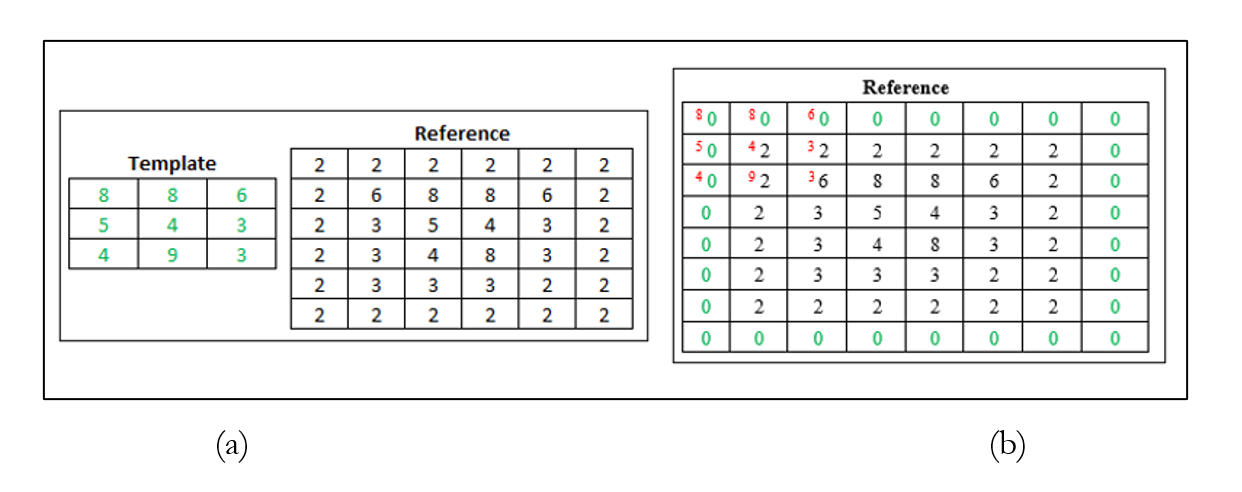
\includegraphics[width=1\columnwidth]{bab3/Gambar/Picture12.png}
		\end{center}
		\vspace{-0.2cm}
		%\rule{\columnwidth}{0.1pt}
		\captionsetup{justification=centering}
		\caption{Template and Referensi Matriks}\label{img:Template-Referensi-Matriks}
	\end{figure}
	%%%%%%%%%%%%%%%%%%%%%%%%%% GAMBAR %%%%%%%%%%%%%%%%%%%%%%%%%%%%%%
	
	Gambar \ref{img:Template-Referensi-Matriks} (a) menunjukkan dua matriks yang digambarkan sebagai template dan referensi gambar sebelum proses pencocokan gambar. Pertama kali proses dimulai, lokasi di tengah template harus diidentifikasi terlebih dahulu, sehingga titik tengah akan jatuh pada piksel referensi pertama seperti yang ditunjukkan pada Gambar \ref{img:Template-Referensi-Matriks} (a). Dalam menemukan titik tengah lokasi template, akan lebih mudah untuk membagi gambar template menjadi dua. Pada contoh template ini, titik tengah lokasi berada pada koordinat (2,2) dengan nilai 4. Pada gambar referensi ditambahkan baris dan kolom dengan nilai nol pada setiap sisi gambar. Jumlah baris dan kolom yang diisi dengan angka nol sama dengan panjang sumbu x dan sumbu y pada template dibagi dua. Gambar \ref{img:Template-Referensi-Matriks} (b) menunjukkan bagaimana gambar template mengisi piksel referensi ketika proses dimulai. Setiap sisi dari gambar referensi berhasil ditambahkan dengan baris dan kolom dengan nilai 0. Dengan menambahkan gambar dengan nilai nol, template tengah dengan mudah ditempatkan pada piksel pertama dari gambar referensi. Untuk setiap lokasi, nilai gambar ditambahkan dan template dijumlahkan dengan menggunakan metode ukuran kemiripan atau \textit{normalized cross correlation} (NCC) dan hasil komputasi disimpan dalam matriks tertentu yang memiliki jumlah gambar referensi yang sama. Akhirnya, matriks dihasilkan setelah semua area gambar diisi. Komputasi gambar digunakan untuk menentukan seberapa tepat template dari area referensi gambar.
	
	\item \textit{Normalized Cross Correlation} (NCC)
	
	Korelasi Silang Ternormalisasi (\textit{Normalized Cross Correlation}, NCC) selalu dipilih karena memiliki keuntungan sebagai ukuran kemiripan yang kuat.  NCC untuk nilai korelasi dengan persamaan sebagai berikut:
	
	$r=\ \frac{\sum_{k=1}^{n}{\left(x_{ik}-\ {\bar{x}}_i\right)\ .\ (x_{jk\ }-{\bar{x}}_i)}}{\sqrt{\left[\sum_{k=1}^{n}{\left(x_{ik}-\ {\bar{x}}_i\right)^2\ .\ \ }\sum_{k=1}^{n}{\left(x_{jk}-\ {\bar{x}}_j\right)^2\ \ }\right]}}$ \hfill (6)\\
	Dengan, xi dan xj adalah rata-rata matriks i dan j yang dapat dihitung dengan:\\
	${\bar{x}}_i=\ \frac{1}{n}\ \sum_{k=1}^{n}x_{ik}$ \hfill (7)\\
	${\bar{x}}_j=\ \frac{1}{n}\ \sum_{k=1}^{n}x_{jk}$ \hfill (8)\\
	
	Keterangan:
	\begin{itemize}
		\item 	$r$ = nilai korelasi antara dua matriks.
		\item $xik$ = nilai piksel ke-k dalam matriks i.
		\item $xjk$ = nilai piksel ke-k dalam matriks j.
		\item ${\bar{x}}_i$ = nilai piksel rata-rata dari matriks i.
		\item ${\bar{x}}_j$ = nilai rata-rata piksel dari matriks j.
		\item n = jumlah piksel dalam sebuah matriks.
	\end{itemize}
	Setelah mendapatkan nilai korelasi antar template, langkah selanjutnya adalah menentukan hasil rata-rata korelasi antar template untuk dijadikan nilai minimum dari nilai acuan yang akan digunakan dalam klasifikasi hasil pengujian pada bagian match template. Perhitungannya sebagai berikut:
	
	${mean\ }_r=\ \frac{(\sum_{r,\ k=1}^{n})}{(\sum_{k=1}^{n})}\ $ \hfill (9)
	
	Keterangan:
	\begin{itemize}
		\item $(\ \sum_{r,\ k=1}^{n})$ = jumlah nilai r dari k-1 hingga n
		
		\item $(\sum_{k=1}^{n})$ = jumlah data dari k-1 to n
	\end{itemize}
	
	Deteksi akhir dari nilai korelasi yang diperoleh, nilai tersebut kemudian dikonversi dalam rentang 0 hingga 255 pada kanal hijau untuk digambarkan dalam bentuk persegi panjang pada koordinat gambar yang terdeteksi pohon.
	
\end{enumerate}

\subsubsection{Penambahan Template}
\hspace{1,2cm}Pada bagian ini, untuk menambahkan gambar template asli, yaitu dengan memutar setiap gambar template sebesar 30 derajat. Hal ini dapat diatur sesuai dengan kebutuhan pengguna. Hal ini dilakukan untuk menambahkan gambar template, sehingga jika mendapatkan gambar yang ternyata dirotasi dari gambar aslinya, maka dapat menemukan kecocokan dari gambar template. Rumusnya sebagai berikut:

$rotations=[i\ast30\ for\ i\ in\ range\ \left(1,4\right)]$ \hfill (10)
Di mana gambar i dirotasi 30 derajat sebanyak 4 kali dari gambar template yang ada.

\subsubsection{Menjalankan Template Matching}
\hspace{1,2cm}	Proses penentuan klasifikasi citra yang telah diuji menggunakan algoritma Template Matching Normal Cross Correlation, seperti pada persamaan (6) pada citra yang akan ditentukan anotasi citranya dan sesuai dengan nilai minimum mean r.

\subsubsection{Analisis Kluster dengan BIRCH}
\hspace{1,2cm}\textit{Balanced Iterative Reducing and Clustering Using Hierarchies} (BIRCH) sebagai algoritma data mining tanpa pengawasan yang digunakan untuk melakukan pengelompokan hirarkis pada kumpulan data yang besar. Algoritma ini menggunakan pengelompokan fitur (feature clustering/FC) dan pengelompokan pohon fitur (CF Tree), dua konsep untuk deskripsi klaster secara umum. BIRCH mampu meningkatkan algoritma dalam melakukan clustering data set yang besar pada kecepatan dan skalabilitas dan sangat cocok untuk menangani masalah pengelompokan data atribut diskrit dan kontinu, seperti piksel yang berdekatan dan menyaring hasil untuk menemukan nilai ambang batas yang lebih baik dari objek yang terdeteksi dari template matching. Objek-objek dalam data set disusun dalam bentuk sub-clustering CF. CF ini kemudian digabungkan menjadi k-kelompok dengan menggunakan prosedur pengelompokan hirarki tradisional. CF adalah tiga informasi yang berisi CF = (N, LS, SS).\\
Keterangan:
\begin{itemize}
	\item N adalah jumlah titik data,
	
	\item LS adalah jumlah nilai X (nilai atribut), 
	
	\item SS adalah jumlah X kuadrat.
	
\end{itemize}

Jika ada 2 CF yang digabungkan, maka teorema:\\
$CF12=(N1+N2,\ {\bar{LS}}_1+\ {\bar{LS}}_2,\ SS1+SS2)$ \hfill (11)

Selanjutnya, untuk mencari lokasi fitur cluster yang cocok untuk digunakan beserta rumus jaraknya. rumus jarak yang digunakan D2 adalah sebagai berikut:

$D2=\ \frac{\sqrt{\left(N_1{SS}_2\right)+\left(N_2{SS}_1\right)-2{LS}_1{LS}_2}}{N_1N_2}$ \hfill (12)

Selanjutnya, untuk dapat menghitung jari-jari daun CF dengan menggunakan rumus:

$R=\ \frac{\sqrt{SS-{(LS)}^2}/n}{n}$ \hfill (13)

Setelah mendapatkan nilai radius dalam kisaran titik tengah gambar, kemudian digunakan threshold. Threshold digunakan pada BIRCH untuk memisahkan objek dari latar belakang pada sebuah citra dengan menggunakan nilai 0,5 sebagai nilai ambang batas atau threshold. Setelah dilakukan perhitungan dengan BIRCH untuk mereduksi atau mengurangi data yang tidak seharusnya masuk, maka data citra ditampilkan dengan ukuran 12 x 12 dengan nilai minimum dari mean r dan citra terdeteksi sebagai citra yang akan dianotasi. Hasil citra juga menampilkan nilai kecocokan dari korelasi yang ditentukan.

\subsubsection{Menjalankan Auto-Annotate Datasets}
\hspace{1,2cm}Proses auto annotation ini merupakan proses dimana mendapatkan data citra (\textit{data collecting}) yang dimiliki, yaitu 205 citra yang telah berhasil dideteksi untuk didapatkan sebagai dataset. Keluaran dari proses ini adalah number, koordinat x, koordinat y, \textit{width}, dan \textit{height} setiap objek yang terdeteksi dari gambar yang disimpan dalam sebuah file berekstensi *.txt. Hasil ini membutuhkan waktu sesuai dengan perangkat yang digunakan. Hasil anotasi dataset ini juga menjadi kebaruan atau \textit{novelty} dalam penelitian ini karena data primer yang diambil secara langsung, serta sudah memiliki anotasi atau label 'oil palm' pada citra pohon kelapa sawit di area lahan. 

\subsubsection{Integrasi Data}
\hspace{1,2cm}Pada tahap ini dilakukan proses menggabungkan atau menyatukan dua dataset, yaitu dataset primer dan sekunder ke dalam satu sumber. Dataset sekunder digunakan layanan roboflow untuk menampung data, dan hasil dari pembangunan dataset dengan anotasi atau pelabelan otomatis yang telah dilakukan, maka diunggah data citra dan file *.txt untuk dapat disesuaikan dengan format data yang sama.

\subsubsection{Format Data}
\hspace{1,2cm}Pada tahap format data ini, salah satu tahap yang sangat penting karena kesuksesan suatu model machine atau deep learning sangat tergantung pada kualitas data yang digunakan untuk pelatihan model tersebut. Pada tahap ini yang dilakukan adalah memeriksa dan memastikan bahwa dataset yang digunakan tidak memiliki nilai yang hilang (yaitu adanya \textit{bounding box}) yang menyatakan bahwa objek tersebut adalah objek kelapa sawit dengan kelas 'oil palm' yang dapat terlihat pada layanan roboflow, kemudian menyesuaikan tipe data pada citra yaitu pada dataset primer dan sekunder sama-sama *.jpg, dan mengurangi dimensi dataset citra dengan melakukan resize citra menjadi 640 x 640 untuk mengurangi \textit{noise} pada data dan menyamakan dataset primer dan sekunder dengan menggunakan layanan roboflow.

\section{Citra untuk Komputasi}
\hspace{1,2cm}	Citra gambar untuk komputasi merupakan kumpulan dari citra dataset primer dan sekunder. Pada tahap ini dataset dikumpulkan dalam satu folder dengan menggunakan layanan Google Drive untuk dapat diakses dan dibagi dalam pelatihan, validasi, dan pengujian. Dataset mengandung 6056 data, yang terbagi ke dalam 78\% data pelatihan, 20\% data validasi dan 2\% data pengujian.

\section{Pelatihan Model CNN}
\hspace{1,2cm}Algoritma CNN model yang digunakan adalah YOLOv7 (sesuai hasil pelatihan dan pengujian) yang divalidasi dengan menggunakan K-Fold Cross-Validation, dimana semua bagian dataset dapat digunakan untuk training dan testing. Teknik ini digunakan untuk evaluasi performance dari model untuk mengurangi overfitting. Langkah awal dalam menggunakan metode cross validation adalah memilih nilai k, kemudian membagi dataset menjadi beberapa nilai k yang digunakan.  Pada penelitian ini menggunakan k = 5, dimana proses ini diulang sebanyak k = 5 kali. K=5, berarti, diberikan dataset and dibagi ke dalam 5 folds yang digunakan untuk menjalankan data pelatihan dan data uji. Model kemudian dilatih pada dataset pelatihan dan divalidasi pada dataset pengujian.  Pada penelitian ini, dipilih nilai k = 5, mengacu pada scikit learn, dengan menerapkan 5-folds. 

Masing-masing setiap fold terdiri dari pelatihan dan pengujian. Data pelatihan merupakan gabungan dari data pelatihan sebanyak 4744 data dan 1187 validasi, untuk data test sebanyak 125 data citra. Setiap fold berisi data ini untuk dapat diketahui pada fold mana hasil model yang dilatih hasilnya lebih baik. 

\section{Optimisasi Parameter}
\hspace{1,2cm}Dalam meningkatkan performa dari model CNN yang digunakan, maka dilakukan optimisasi parameter. Optimisasi parameter pada penelitian ini menggunakan epoch, batch size, initial learning rate, final one cycle learning rate, momentum, dan weight decay sebagai optimizer weight decay seperti pada Tabel \ref{tbl:Optimisasi-Parameter}.

%%%%%%%%%%%%%%%%%%%%%%%TABEL SEDERHANA%%%%%%%%%%%%%%%%%%%%%%%%%
\begin{singlespace}
	\begin{table}[H]
		\centering
		\caption{Optimisasi Parameter}
		\label{tbl:Optimisasi-Parameter}
		\begin{tabular}{|c|c|}
			\hline
			\rowcolor[HTML]{D9D9D9} 
			Parameter    & Nilai         \\ \hline
			lr0          & 0.01 (1E-2)   \\ \hline
			rf           & 0.1           \\ \hline
			Momentum     & 0.937         \\ \hline
			Weight decay & 0.0005 (5e-4) \\ \hline
			Epoch        & 30            \\ \hline
			Batch size   & 16            \\ \hline
		\end{tabular}
	\end{table}
\end{singlespace}
%%%%%%%%%%%%%%%%%%%%%%%TABEL SEDERHANA%%%%%%%%%%%%%%%%%%%%%%%%%

Parameter yang digunakan diantaranya adalah learning rate dengan nilai 0.01 \textit{stochastic gradient descent} (SGD). Learning rate ini hyperparameter yang paling penting ketika mengonfigurasi neural network. Hal sangat penting untuk mengetahui bagaimana menyelidiki efek dari laju pembelajaran pada kinerja model dan untuk membangun intuisi tentang dinamika laju pembelajaran pada perilaku model. Nilai \textit{learning rate} yang terlalu kecil dapat menyebabkan proses pelatihan yang lama dan bisa \textit{stuck} atau berhenti, sedangkan nilai yang terlalu besar dapat menyebabkan pembelajaran set bobot yang tidak optimal menjadi terlalu cepat atau proses pelatihan yang tidak stabil. Penelitian ini menggunakan learning rate dari SGD 0.001 karena metode optimasi adaptif lainnya diketahui memiliki generalisasi yang buruk dibandingkan dengan SGD. Metode lainnya cenderung berkinerja baik pada data pelatihan tetapi, tidak saat data pengujian. Parameter yang digunakan berikutnya adalah momentum. Momentum digunakan sebagai metode yang membantu mempercepat vektor gradien ke arah yang benar, sehingga menghasilkan konvergen yang lebih cepat, atau dengan kata lain sebagai pengoptimal yang meminimalisir dampak noise dalam konvergensi ke bobot optimal.

Pada penelitian ini menggunakan epoch sebesar 30 epoch karena sebelumnya sudah diujicoba kan dengan epoch 55 dan 50, maka tidak bisa berjalan hingga selesai karena adanya \textit{out of memory} dan batas GPU dari Google, sehingga digunakan 30 epoch dengan batch size 16. Epoch menjadi penting karena hyperparameter yang menentukan berapa kali algoritma \textit{deep learning} bekerja melewati seluruh dataset. Batch size yang digunakan adalah 16, ini mengacu pada jumlah contoh data pelatihan yang digunakan dalam satu iterasi.

\section{Menjalankan Model CNN}
\hspace{1,2cm}Pada tahap ini menjalankan hasil training dan test dari dataset yang sudah disiapkan dengan menggunakan parameter tercantum pada Tabel 3.4 dengan YOLOv7 menggunakan teknik K-Fold Cross-validation untuk evaluasi model untuk setiap segmen. Pada tahap ini, model dijalankan dengan menggunakan YOLOv7, yang dimana algoritma ini bekerja berdasarkan empat pendekatan seperti pada alur diagram Gambar \ref{img:Cara-Kerja-Pendekatan-Algoritma-YOLOv7}.

%%%%%%%%%%%%%%%%%%%%%%%%%% GAMBAR %%%%%%%%%%%%%%%%%%%%%%%%%%%%%%
\begin{figure}[H]
	\vspace{-0.1cm}
	%\rule{\columnwidth}{0.1pt}
	\begin{center}
		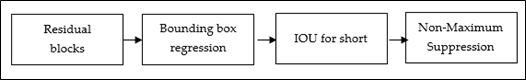
\includegraphics[width=1\columnwidth]{bab3/Gambar/Picture13.png}
	\end{center}
	\vspace{-0.2cm}
	%\rule{\columnwidth}{0.1pt}
	\captionsetup{justification=centering}
	\caption{Cara Kerja Pendekatan Aloritma YOLOv7}\label{img:Cara-Kerja-Pendekatan-Algoritma-YOLOv7}
\end{figure}
%%%%%%%%%%%%%%%%%%%%%%%%%% GAMBAR %%%%%%%%%%%%%%%%%%%%%%%%%%%%%%

Langkah pertama ini dimulai dengan membagi gambar asli menjadi sel grid S x S dengan bentuk yang sama. Setiap sel grid bertanggung jawab untuk menentukan dan memprediksi lokasi kelas dan nilai probabilitas/\textit{confidence} objek tersebut. Langkah selanjutnya adalah menentukan kotak pembatas yang sesuai dengan persegi panjang yang menyoroti semua objek dalam gambar. YOLO menentukan sifat-sifat kotak pembatas ini menggunakan modul regresi tunggal dalam bentuk berikut, di mana Y adalah representasi vektor akhir dari setiap kotak pembatas.

Y = [pc, bx, by, bh, bw, c1, c2] \hfill (14)

Keterangan:
\begin{itemize}
	\item pc: sesuai dengan skor probabilitas dari sisi yang berisi objek
	
	\item bx, by: koordinat tengah x dan y dari pusat kotak pembatas (bounding box)
	
	\item bh, bw: tinggi dan lebar kotak pembatas.
	
	\item c1 dan c2: berhubungan dengan kelas (dalam penelitian ini menggunakan 1 kelas, yaitu \textit{oil palm})
\end{itemize}

Sering kali, satu objek dalam sebuah gambar dapat memiliki beberapa kandidat kotak grid untuk prediksi, meskipun tidak semuanya relevan. Tujuan \textit{Interception of Union} (IOU) (nilai antara 0 dan 1) untuk membuang kotak-kotak tersebut dan hanya menyimpan kotak-kotak yang relevan, kotak ini lah yang nantinya menjadi \textit{bounding box} yaitu klasifikasi kelas dan juga lokalisasi, yaitu titik tengah koordinat dari \textit{bounding box} tersebut. Terkadang IoU menetapkan nilai ambang batas untuk IoU yang tidak cukup untuk sebuah objek, Di sinilah, dapat menggunakan non-maximum suppresion untuk menyimpan hanya kotak dengan nilai probabilitas deteksi tertinggi, sehingga kotak tersebut dapat menentukan atau mendeteksi kelas apa dalam \textit{bounding box} tersebut. Hasil dari menjalankan model ini, didapatkan hasil evaluasi kualitas model terbaik, dan hasil tersebut akan dipilih sebagai model terbaik.

Pada Gambar \ref{img:Skema-Diagram-Algoritma-YOLO} skema diagram dari algoritma YOLOv7 yang digunakan dalam penelitian ini, bagaimana dataset dapat dideteksi sebagai oil palm.

%%%%%%%%%%%%%%%%%%%%%%%%%% GAMBAR %%%%%%%%%%%%%%%%%%%%%%%%%%%%%%
\begin{figure}[H]
	\vspace{-0.1cm}
	%\rule{\columnwidth}{0.1pt}
	\begin{center}
		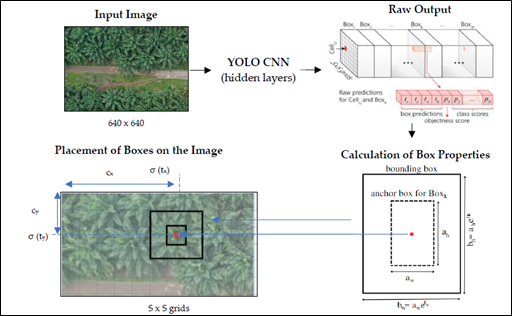
\includegraphics[width=1\columnwidth]{bab3/Gambar/Picture14.png}
	\end{center}
	\vspace{-0.2cm}
	%\rule{\columnwidth}{0.1pt}
	\captionsetup{justification=centering}
	\caption{Skema Diagram Algoritma YOLO}\label{img:Skema-Diagram-Algoritma-YOLO}
\end{figure}
%%%%%%%%%%%%%%%%%%%%%%%%%% GAMBAR %%%%%%%%%%%%%%%%%%%%%%%%%%%%%%

Pada penelitian ini dataset yang digunakan sebagai \textit{input image} atau data citra yang masuk ke YOLO (\textit{neural network}) dengan resolusi 640 x 640. Artinya, ukuran gambar yang lebih besar diubah ke resolusi 640 x 640 yang merupakan ukuran \textit{default} dari YOLO. Hal ini dilakukan untuk mengurangi resiko kehilangan akurasi prediksi yang baik. Berdasarkan Gambar \ref{img:Cara-Kerja-Pendekatan-Algoritma-YOLOv7} bahwa kalkulasi box properties menjadi penting untuk mendapatkan objek yang berhasil dideteksi dengan tampilanya bounding box, dan diketahui titik tengah (x, y) atau lokasi dari setiap objek kelas oil palm yang berhasil dideteksi.

Setelah berhasil mengetahui bagaimana diagram skema kerja algoritma YOLO untuk mendeteksi objek \textit{oil palm} pada data citra, maka dibutuhkan evaluasi model performance dari model yang dijalankan dalam penelitian ini. Evaluasi performance untuk mendapatkan model terbaik dengan evaluasi performa dari sebuah model pendeteksian objek biasanya menggunakan precision, recall, dan F1-score serta \textit{best Mean Average Precision} atau yang dikenal dengan best mAP yang umumnya digunakan untuk menganalisis kinerja sistem deteksi dan segmentasi objek.

Precision = $\frac{(TP)}{(\left(TP\right)+\left(FP\right))}$ \hfill (15)

Recall = $\frac{(TP)}{(\left(TP\right)+\left(FN\right))}$ \hfill (16)

F1-Score = 2 x $\frac{Precision\ x\ Recall}{Precision+\ Recall}$ \hfill (17)

$mAP=\ \frac{1}{N}\sum_{i=1}^{N}{AP}_{i}$ \hfill (18)
	
Keterangan:
\begin{itemize}
	\item TP: True Positive untuk jumlah piksel yang benar diklasifikasikan sebagai pohon kelapa sawit
	
	\item FP: False Positive untuk jumlah piksel yang tidak benar diklasifikasikan sebagai pohon kelapa sawit. 
	
	\item FN: False Negative untuk jumlah piksel yang tidak benar diklasifikasikan sebagai latar belakang. 
	
\end{itemize}

Pada tahap ini model yang dijalankan dengan menggunakan sarana penelitian dengan menggunakan mesin untuk komputasi dengan mengakses Google Colab Pro (DGX-SM4-A100, 40 GB) dan mesin (DGX-A100, 20 GB) milik Universitas Gunadarma.

\section{Hasil Deteksi dan Penghitungan Akhir}
\hspace{1,2cm}Tahap ini menggunakan sebuah web framework react js untuk menerapkan hasil best model dari performance terbaik untuk dapat digunakan pada citra satelit realtime yang terhubung dengan Google Maps API. Untuk model terbaik dari YOLOv7 harus dikonversi yang bisa dikenali dalam backend pada pengembangan sistem. Format yang digunakan adalah \textit{open neural network exchange} (ONNX) yang merupakan untuk merepresentasikan model pembelajaran mesin dan format file yang umum untuk memungkinkan menggunakan model dengan berbagai kerangka kerja, alat, waktu proses, dan compiler. File onnx ini diletakkan di server dengan menggunakan FastAPI sebagai backend. Dalam mendapatkan titik tengah koordinat latitude dan longitude setiap object dari bounding box, dibutuhkan titik tengah awal sebagai titik koordinat latitude dan longitude kunci, sehingga bisa didapatkan titik tersebut yang di \textit{request} ke Google Maps API dengan menggunakan bantuan library mapping dari leaflet js.

Adapun diagram alur hasil deteksi dan penghitungan akhir pada Gambar \ref{img:Diagram-ALur-Hasil-Deteksi-dan-Perhitungan-Akhir}.

%%%%%%%%%%%%%%%%%%%%%%%%%% GAMBAR %%%%%%%%%%%%%%%%%%%%%%%%%%%%%%
\begin{figure}[H]
	\vspace{-0.1cm}
	%\rule{\columnwidth}{0.1pt}
	\begin{center}
		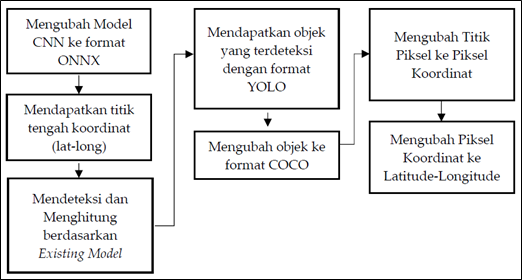
\includegraphics[width=1\columnwidth]{bab3/Gambar/Picture15.png}
	\end{center}
	\vspace{-0.2cm}
	%\rule{\columnwidth}{0.1pt}
	\captionsetup{justification=centering}
	\caption{Diagram Alur Hasil Deteksi dan Penghitungan Akhir}\label{img:Diagram-ALur-Hasil-Deteksi-dan-Perhitungan-Akhir}
\end{figure}
%%%%%%%%%%%%%%%%%%%%%%%%%% GAMBAR %%%%%%%%%%%%%%%%%%%%%%%%%%%%%%

Hasil objek yang dideteksi yang ditandai dengan bounding box, masih dengan menggunakan format YOLO. \textit{Bounding box} yang dihasilkan tersebut merepresentasikan posisi relative dari titik tengah \textit{bounding box} (x,y) dan width, serta height dari objek yang dideteksi, sedangkan format COCO merepresentasikan piksel asli \textit{bounding box} dari citra gambar tersebut. Terdapat perbedaan titik-titik bounding box antara format YOLO dengan COCO. Pada format COCO bounding box dengan format <top left x, top left y, width, height>, dimana lebar dan tinggi adalah dimensi dari \textit{bounding box}. Perbedaan format COCO dan YOLO seperti pada Gambar \ref{img:Bounding-Box-Pada-COCO-dan-YOLO}. 

%%%%%%%%%%%%%%%%%%%%%%%%%% GAMBAR %%%%%%%%%%%%%%%%%%%%%%%%%%%%%%
\begin{figure}[H]
	\vspace{-0.1cm}
	%\rule{\columnwidth}{0.1pt}
	\begin{center}
		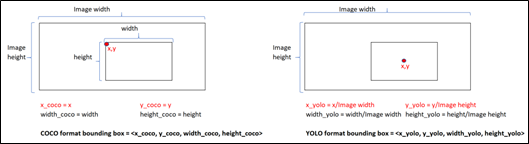
\includegraphics[width=1\columnwidth]{bab3/Gambar/Picture16.png}
	\end{center}
	\vspace{-0.2cm}
	%\rule{\columnwidth}{0.1pt}
	\captionsetup{justification=centering}
	\caption{\textit{Bounding Box} pada COCO dan YOLO format}\label{img:Bounding-Box-Pada-COCO-dan-YOLO}
\end{figure}
%%%%%%%%%%%%%%%%%%%%%%%%%% GAMBAR %%%%%%%%%%%%%%%%%%%%%%%%%%%%%%

Berdasarkan Gambar \ref{img:Bounding-Box-Pada-COCO-dan-YOLO}, maka persamaan untuk mengubah format dari YOLO ke COCO, adalah:

$x_{coco}=x_{yolo}\ast image\ width$ \hfill(19)

$y_{coco}=y_{yolo}\ast image\ height$ \hfill(20)

$w_{coco}\ =w_{yolo}\ast image\ width-x_{coco}$ \hfill(21)

$h_{coco}\ =h_{yolo}\ast image\ height-y_{coco}$ \hfill(22)

$x_{center}=x+\frac{w}{2} $ \hfill(23)

$y_{center}=y+\frac{h}{2}$ \hfill(24)

Selanjutnya, setelah didapatkan titik dari format COCO, kemudian dilanjutkan dengan dikonversi untuk menghitung piksel koordinat dari latitude-longitude awal ke titik tengah ke piksel koordinat dari web mercator projection pada zoom 0 (base world map) sebesar ukuran 256 x 256 piksel. Persamaan berikut ini menempatkan sumbu x proyeksi pada khatulistiwa dan sumbu y pada bujur $\lambda 0$, di mana $\lambda O$ adalah garis bujur, di mana y adalah proyeksi Mercator dari garis lintang dan $\varphi$ adalah garis lintang dalam radian. $\lambda$ adalah longitude dan $\phi$ adalah latitude.

$\mathbit{x}=\mathbit{R}(\mathbit{\lambda}-\ \mathbit{\lambda}_\mathbf{0})\, y = R ln[\mathbf{tan}({\frac{\mathbit{\pi}}{\mathbf{4}}+}\frac{\mathbit{\phi}}{\mathbf{2}})$ \hfill (25)

Berikutnya mengubah pixel coordinates menjadi latitude-longitude untuk setiap titik tengah dari bounding box tersebut dengan menggunakan invers transformation dari persamaan 26. Ekspresi pada kanan kedua equation menggambarkan longitude, dan latitude pada sisi kiri, sedangkan nanti pada penulisan titik koordinat, dituliskan latitude-longitude.

$\mathbit{\lambda}=\ \mathbit{\lambda}_\mathbf{0}+\ \frac{\mathbit{x}}{\mathbit{R}}\ , \mathbit{\phi} = 2 tan-1 [exp(yR]-π2)$ \hfill (26)

Dari persamaan 25 dan 26, maka dihasilkan titik koordinat latitude dan longitude dari setiap bounding box yang merepresentasikan keberadaan objek, dan untuk menghitung banyaknya pohon didasarkan pada banyaknya yang terdeteksi objek pohon kelapa sawit tersebut. Catatan bahwa yang digunakan untuk nilai $\pi$ adalah 3.141592653589793.

Penerapan hasil deteksi dan penghitungan akhir, diterapkan pada diagram sistem arsitektur Gambar \ref{img:Diagram-Arsitektur-Sistem}.

%%%%%%%%%%%%%%%%%%%%%%%%%% GAMBAR %%%%%%%%%%%%%%%%%%%%%%%%%%%%%%
\begin{figure}[H]
	\vspace{-0.1cm}
	%\rule{\columnwidth}{0.1pt}
	\begin{center}
		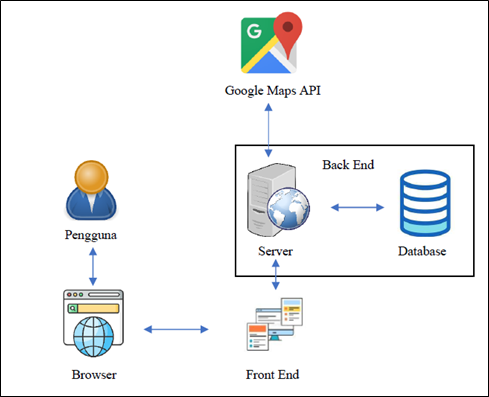
\includegraphics[width=1\columnwidth]{bab3/Gambar/Picture17.png}
	\end{center}
	\vspace{-0.2cm}
	%\rule{\columnwidth}{0.1pt}
	\captionsetup{justification=centering}
	\caption{Diagram Arsitektur Sistem}\label{img:Diagram-Arsitektur-Sistem}
\end{figure}
%%%%%%%%%%%%%%%%%%%%%%%%%% GAMBAR %%%%%%%%%%%%%%%%%%%%%%%%%%%%%%

Gambar \ref{img:Diagram-Arsitektur-Sistem}. merupakan diagram sistem arsitektur pada penerapan penelitian ini. Penguna untuk dapat mengakses melalui browser untuk dapat membuka laman penerapan sistem dari mendeteksi dan menghitung pohon kelapa sawit, serta mengetahui letak titik koordinat setiap pohon kelapa sawit tersebut. Pengguna dapat menggunakan perangkat lunak atau aplikasi yang dikenal dengan browser, seperti Google Chrome untuk dapat meminta laman yang dapat memberikan tampilan antarmuka.

Laman yang diakses atau diminta, memiliki tampilan antarmuka atau yang dikenal dengan \textit{user interface}. Front end pada penerapan sistem ini menggunakan react js. React js digunakan untuk dapat membuat \textit{user interface} pada tampilan berbasis web dan berisi library kode javascript yang memudahkan dalam web development. Tampilan antarmuka merupakan permintaan dan menampilkan ke pada server.

Server pada penelitian ini menggunakan FastAPI. FastAPI digunakan karena sebuah web framework untuk membangun sebuah \textit{application programming interface} (API) untuk produksi atau model \textit{machine learning}. Model CNN ini-lah yang diletakkan pada server untuk dapat mengenali objek yang akan diprediksi melalui gambar yang diminta melalui maps atau pemetaan satelit. Hasil prediksi merupakan data yang harus disimpan. Penyimpanan basis data menggunakan PostgreSQL. PostgreSQL basis data yang digunakan pada web app, aplikasi mobile, dan aplikasi analytics. Aplikasi yang membutuhkan pengolahan data yang lebih kompleks akan lebih cocok menggunakan PostgreSQL.

Tampilan Maps yang ditampilkan pada front end merupakan hasil dari permintaan yang terintegrasi terhubung dari Google Maps API. Dari Google Maps API maka dapat melihat sebuah peta datar (\textit{mercator projection}) untuk dapat dipetakan suatu lahan pada area tertentu dan kemudian dideteksi citra kelapa sawit dan kemudian diketahui jumlah, serta letak posisi dari pohon kelapa sawit tersebut yang berguna untuk hasil pemantauan dari pohon kelapa sawit. Berikut ini komponen implementasi dalam prototype perangkat lunak Tabel \ref{tbl:Komponen-Implementasi-Prototype}. dan perangkat keras Tabel \ref{tbl:Komponen-Implementasi-Prototype-Perangkat-Keras}. dalam menerapkan model terbaik di dalam prototype berbasis web.

%%%%%%%%%%%%%%%%%%%%%%%TABEL SEDERHANA%%%%%%%%%%%%%%%%%%%%%%%%%
\begin{singlespace}
	\begin{table}[H]
		\centering
		\caption{Komponen Implementasi Prototype Perangkat Lunak}
		\label{tbl:Komponen-Implementasi-Prototype}
		\begin{tabular}{|p{1cm}|p{4cm}|p{7cm}|}
			\hline
			\rowcolor[HTML]{D9D9D9} 
			No                 & Komponen                  & Keterangan                                                                                                                                                                                                                                                                                                                                        \\ \hline
			1                  & Browser                   & Google Chrome v. 113.0.5672.64                                                                                                                                                                                                                                                                                                                    \\ \hline
			2                  & Google Maps API           & Layanan Google Static Map API                                                                                                                                                                                                                                                                                                                     \\ \hline
			3                  & Back End                  &                                                                                                                                                                                                                                                                                                                                                   \\ \hline
			& a. Web Server FastAPI     & v.0.85.0 (FastAPI adalah sebuah web framework untuk membangun sebuah API yang berbahasa Python).                                                                                                                                                                                                                                                  \\ \cline{2-3} 
			& b. SQLAlchemy             & v.1.4.41 (Library yang memfasilitasi komunikasi antara program Python dan database. Library ini digunakan sebagai alat Object Relational Mapper (ORM) yang menerjemahkan kelas-kelas Python ke tabel-tabel di database relasional dan secara otomatis mengubah panggilan fungsi menjadi pernyataan SQL).                                          \\ \cline{2-3} 
			& c. numpy                  & v.1.24.1 (NumPy (Numerical Python) adalah library Python yang fokus pada scientific computing. Library ini digunakan untuk melakukan perhitungan saintifik, seperti matriks, aljabar, dan statistik). Pada pengolahan gambar digunakan untuk manipulasi dan transformasi gambar, seperti memotong, merotasi, membalik dan mengubah ukuran gambar. \\ \cline{2-3} \hline
		\end{tabular}
	\end{table}
\end{singlespace}
%%%%%%%%%%%%%%%%%%%%%%%TABEL SEDERHANA%%%%%%%%%%%%%%%%%%%%%%%%%

%%%%%%%%%%%%%%%%%%%%%%%TABEL SEDERHANA%%%%%%%%%%%%%%%%%%%%%%%%%
\begin{singlespace}
	\begin{table}[H]
		\centering
		%\caption{Komponen Implementasi Prototype Perangkat Lunak}
		%\label{tbl:Komponen-Implementasi-Prototype}
		\begin{tabular}{|p{1cm}|p{4cm}|p{7cm}|}
			\hline
			\rowcolor[HTML]{D9D9D9} 
			No                 & Komponen                  & Keterangan                                                                                                                                                                                                                                                                                                                                        \\ \hline
			& d. onnxruntime            & v.1.13.1. (Format model machine learning yang dapat dioperasikan pada berbagai platform dan dapat dijalankan pada berbagai platform seperti web)                                                                                                                                                                                                  \\ \cline{2-3} 
			& e. opencv-python-headless & v.4.6.0.66 (Library OpenCV untuk Python yang digunakan untuk pengolahan gambar, seperti pengolahan citra, deteksi objek, dan visi komputer)                                                                                                                                                                                                       \\ \cline{2-3} 
			\multirow{-6}{*}{} & f. DBMS: PostgreSQL       & v.14.7 (Sistem manajemen basis data yang dapat menyimpan data dalam bentuk array atau JSON dan berguna dalam Machine Learning)                                                                                                                                                                                                                    \\ \hline
			4                  & Front End                 &                                                                                                                                                                                                                                                                                                                                                   \\ \hline
			& a. react js               & v.18.2.0 (Digunakan untuk dapat membuat user interface pada tampilan berbasis web dan berisi library kode javascript)                                                                                                                                                                                                                             \\ \cline{2-3} 
			& b. tailwindcss            & v.3.2.4 (Framework CSS yang digunakan untuk mempercepat pengembangan tampilan (UI) web)                                                                                                                                                                                                                                                           \\ \cline{2-3}
			& c. typescript             & v.4.9.3 (Bahasa pemrograman yang digunakan untuk mengembangkan aplikasi Machine Learning berbasis web dengan menggunakan framework react)                                                                                                                                                                                                         \\ \cline{2-3} 
			\multirow{-4}{*}{} & d. leaflet js             & v.1.9.3 (library JavaScript yang digunakan untuk memvisualisasikan peta interaktif pada halaman web dan dapat digunakan dalam konteks Machine Learning untuk memvisualisasikan data geospasial dan membuat aplikasi peta interaktif)                                                                                                              \\ \hline
		\end{tabular}
	\end{table}
\end{singlespace}
%%%%%%%%%%%%%%%%%%%%%%%TABEL SEDERHANA%%%%%%%%%%%%%%%%%%%%%%%%%

%%%%%%%%%%%%%%%%%%%%%%%TABEL SEDERHANA%%%%%%%%%%%%%%%%%%%%%%%%%
\begin{singlespace}
	\begin{table}[H]
		\centering
		\caption{Komponen Implementasi Prototype Perangkat Keras}
		\label{tbl:Komponen-Implementasi-Prototype-Perangkat-Keras}
		\begin{tabular}{|p{1cm}|p{4cm}|p{7cm}|}
			\hline
			\rowcolor[HTML]{D9D9D9} 
			No & Layanan                       & Keterangan                                                                                                                                                                      \\ \hline
			1  & Back End                      &                                                                                                                                                                                 \\ \hline
			& Layanan Google Compute Engine & \begin{tabular}[c]{@{}l@{}}Tipe Mesin: n2-standard-2\\    vCPUs: 2 Core (@ 4GB)\\    CPU Platform: Intel Cascade Lake\\    \\ RAM: 8 GB \\    Architecture: x86/64\end{tabular} \\ \hline
			2  & Front End                     &                                                                                                                                                                                 \\ \hline
			& Layanan Google Compute Engine & \begin{tabular}[c]{@{}l@{}}Tipe Mesin: e2-medium \\    vCPU: 2 Core (@ 4GB) \\    CPU: Platform: Intel Broadwell\\    RAM: 4 GB\\    Architecture: x86/64\end{tabular}          \\ \hline
			\end{tabular}
	\end{table}
\end{singlespace}
%%%%%%%%%%%%%%%%%%%%%%%TABEL SEDERHANA%%%%%%%%%%%%%%%%%%%%%%%%%